\documentclass[12pt, a4paper]{article}
\usepackage[margin=1in]{geometry}
\usepackage{../auxiliary/utilities/preamble}

\newcommand{\titulo}{Transformadas de Lagrange}
\newcommand{\fecha}{11 de febrero de 2024}

\begin{document}
\sffamily
\begin{titlepage}
    \begin{center}
        
\includegraphics[width=0.15\textwidth]{../auxiliary/assets/unam.png}
        \hspace{0.6\textwidth}
        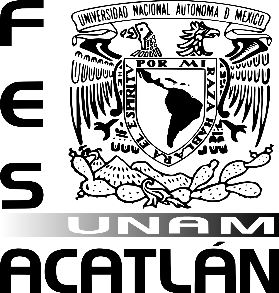
\includegraphics[width=0.15\textwidth]{../auxiliary/assets/fes.png}

        \vspace*{5cm}
        \LARGE
        \textbf{\titulo}

        \vspace{1cm}
        \large
        Camargo Badillo Luis Mauricio \\
        \vspace{1.5cm}
        \textit{\fecha}

        \vfill

        \vspace{0.5cm}
        Ecuaciones Diferenciales II \\
        Oscar Gabriel Caballero Martínez \\
        Grupo 2602 \\
        \textbf{Matemáticas Aplicadas y Computación}\\
    \end{center}
\end{titlepage}


\newpage

\setcounter{section}{7}
\section{\texorpdfstring{\(f(t)=\cos(t)\)}{f (t) = cos (t)}}

Calculamos la transformada de Lagrange de \(f(t) = \cos(t)\):
\begin{align*}
	\mathcal{L}\{\cos (t)\} &= \int_{0}^{\infty} e^{-st} \cos(t)\ dt \\
	&= \lim_{b \to \infty} \int_{0}^{b} e^{-st} \cos(t)\ dt
\end{align*}
Integrando por partes, utilizando \(u = \cos(t) \implies du = -\sin(t)\ dt\) y \(dv = e^{-st}\ dt \implies v = -\frac{1}{s} e^{-st}\), obtenemos:
\begin{align*}
	&= \lim_{b \to \infty} \left[ \left. \frac{-\cos (t) e^{-st}}{s} \right|_{0}^{b} - \frac{1}{s} \int_{0}^{b} e^{-st} \sin (t) \ dt \right] \\
	&= \lim_{b \to \infty} \left[ - \frac{\cos (b) e^{-sb}}{s} + \frac{\cos (0) e^{0}}{s} \right] - \lim_{b \to \infty} \left[ \frac{1}{s} \int_{0}^{b} e^{-st} \sin (t) \ dt \right] \\
	&= \frac{1}{s} - \lim_{b \to \infty} \left[ \frac{1}{s} \int_{0}^{b} e^{-st} \sin (t) \ dt \right] \\
	&= \frac{1}{s} - \frac{1}{s} \lim_{b \to \infty} \int_{0}^{b} e^{-st} \sin (t) \ dt
\end{align*}
Una vez más, integrando por partes con \(u = \sin (t) \implies du = \cos (t)\ dt\) y \(dv = e^{-st}\ dt \implies v = -\frac{1}{s} e^{-st}\), tenemos:
\begin{align*}
	&= \frac{1}{s} - \frac{1}{s} \lim_{b \to \infty} \left[ \left. \frac{-\sin (t) e^{-st}}{s} \right|_{0}^{b} + \frac{1}{s} \int_{0}^{b} e^{-st} \cos (t)\ dt \right] \\
	&= \frac{1}{s} - \frac{1}{s} \lim_{b \to \infty} \left[ - \frac{\sin (b) e^{-sb}}{s} + \frac{\sin (0) e^{0}}{s} \right] + \lim_{b \to \infty} \left[ \frac{1}{s} \int_{0}^{b} e^{-st} \cos (t)\ dt \right] \\
	&= \frac{1}{s} - \frac{1}{s} \lim_{b \to \infty} \left[ \frac{1}{s} \int_{0}^{b} e^{-st} \cos (t)\ dt \right] \\
	&= \frac{1}{s} - \frac{1}{s^{2}} \lim_{b \to \infty} \int_{0}^{b} e^{-st} \cos (t) \ dt
\end{align*}
Observemos que:
\begin{align*}
	\lim_{b \to \infty} \int_{0}^{b} e^{-st} \cos (t) \ dt &= \frac{1}{s} - \frac{1}{s^{2}}\lim_{b \to \infty} \int_{0}^{b} e^{-st} \cos (t) \ dt
\end{align*}
Estableciendo \(a = \lim_{b \to \infty} \int_{0}^{b} e^{-st} \cos (t) \ dt\), tenemos:
\begin{align*}
	a &= \frac{1}{s} - \frac{1}{s ^{2}} a \\
	\implies a + \frac{1}{s ^{2}} a &= \frac{1}{s} \\
	\implies a \left(\frac{1}{s ^{2}} + 1 \right) &= \frac{1}{s} \\
	\implies a \left( \frac{1+s ^{2}}{s ^{2}} \right) &= \frac{1}{s} \\
	\implies a &= \frac{s ^{2}}{s(1+s ^{2})} \\
	\implies a &= \frac{s}{s ^{2} + 1} \\
	\implies \lim_{b \to \infty} \int_{0}^{b} e^{-st} \cos (t) \ dt &= \frac{s}{s ^{2} + 1} \\
	\implies \int_{0}^{\infty} e^{-st} \cos (t) \ dt &= \frac{s}{s ^{2} + 1}
\end{align*}
Por lo tanto, finalmente:
\[
	\mathcal{L}\{\cos (t)\} = \frac{s}{s ^{2} + 1}
\]


\setcounter{section}{10}
\section{\texorpdfstring{\(f(t)=e^{4t}\)}{f (t) = e (4t) }}

Calculamos la transformada de Lagrange de \(f(t) = e^{4t}\):
\begin{align*}
	\mathcal{L}\{e^{4t}\} &= \int_{0}^{\infty} e^{-st} e^{4t}\ dt \\
	&= \int_{0}^{\infty} e^{(4-s)t} \ dt \\
	&= \lim_{b \to \infty} \int_{0}^{b} e^{(4-s)t} \ dt
\end{align*}
Sustituyamos con \(u = (4-s) t \implies du = 4-s\ dt\):
\begin{align*}
	&= \frac{1}{4-s} \lim_{b \to \infty} \int_{0}^{(4-s)b} e^{u} \ du \\
	&= \frac{1}{4-s} \lim_{b \to \infty} \left. \left( e^{u} \right)  \right|_{0}^{(4-s)b} \\
	&= \frac{1}{4-s} \lim_{b \to \infty} \left( e^{(4-s)b} - e^{0} \right) \\
	&= \frac{1}{4-s} \left[ \lim_{b \to \infty} e^{(4-s)b} - 1 \right]
\end{align*}
Cuando \(s > 4 \implies (4-s) < 0\), por lo que podemos escribir:
\begin{align*}
	&= \frac{1}{4-s} \left[ \lim_{b \to -\infty} e^{b} - 1 \right] \\
	&= \frac{1}{4-s} (0 - 1) \\
	&= \frac{1}{s-4}
\end{align*}
Así, finalmente obtenemos que:
\[
	\mathcal{L}\{e^{4t}\} = \frac{1}{s-4} \qquad s > 4
\]

\section{\texorpdfstring{\(f(t)=e^{-2t}\)}{f (t) = e (-2t)}}

Calculamos la transformada de Lagrange de \(f(t) = e^{-2t}\):
\begin{align*}
	\mathcal{L}\{e^{-2t}\} &= \int_{0}^{\infty} e^{-st} e^{-2t}\ dt \\
	&= \int_{0}^{\infty} e^{(-2-s)t} \ dt \\
	&= \lim_{b \to \infty} \int_{0}^{b} e^{(-2-s)t} \ dt
\end{align*}
Sustituyamos con \(u = (-2-s) t \implies du = -2-s\ dt\):
\begin{align*}
	&= \frac{1}{-2-s} \lim_{b \to \infty} \int_{0}^{(-2-s)b} e^{u} \ du \\
	&= \frac{1}{-2-s} \lim_{b \to \infty} \left. \left( e^{u} \right)  \right|_{0}^{(-2-s)b} \\
	&= \frac{1}{-2-s} \lim_{b \to \infty} \left( e^{(-2-s)b} - e^{0} \right) \\
	&= \frac{1}{-2-s} \left[ \lim_{b \to \infty} e^{(-2-s)b} - 1 \right]
\end{align*}
Cuando \(s > -2 \implies (-2-s) < 0\), por lo que podemos escribir:
\begin{align*}
	&= \frac{1}{-2-s} \left[ \lim_{b \to -\infty} e^{b} - 1 \right] \\
	&= \frac{1}{-2-s} (0 - 1) \\
	&= \frac{1}{s+2}
\end{align*}
Así, finalmente obtenemos que:
\[
	\mathcal{L}\{e^{-2t}\} = \frac{1}{s+2} \qquad s > -2
\]

\setcounter{section}{13}
\section{\texorpdfstring{\(f(t)=\sinh(3t)\)}{f (t) = sinh (3t)}}

Calculamos la transformada de Lagrange de \(f(t) = \sinh(3t)\):
\begin{align*}
	\mathcal{L}\{\sinh(3t)\} &= \int_{0}^{\infty} e^{-st} \sinh(3t) \ dt
\end{align*}
Recordemos que \(\sinh(u) = \frac{1}{2} (e^{u} - e^{-u})\), así que:
\begin{align*}
	&= \frac{1}{2} \int_{0}^{\infty} e^{-st} (e^{3t} - e^{-3t}) \ dt \\
	&= \frac{1}{2} \left[ \int_{0}^{\infty} e^{(3-s)t} - e^{(-3-s)t} \ dt \right] \\
	&= \frac{1}{2} \left[ \int_{0}^{\infty} e^{(3-s)t} \ dt - \int_{0}^{\infty} e^{(-3-s)t} \ dt \right] \\
	&= \frac{1}{2} \lim_{b \to \infty} \left[ \int_{0}^{b} e^{(3-s)t} \ dt - \int_{0}^{b} e^{(-3-s)t} \ dt \right]
\end{align*}
Sustituyendo con \(u = (3-s)t \implies du = 3-s\ dt\) y \(v = (-3-s)t \implies dv = -3-s\ dt\), obtenemos:
\begin{align*}
	&= \frac{1}{2} \lim_{b \to \infty} \left[ \frac{1}{3-s} \int_{0}^{(3-s)b} e^{u} \ du - \frac{1}{-3-s} \int_{0}^{(-3-s)b} e^{u} \ du \right] \\
	&= \frac{1}{2} \lim_{b \to \infty} \left[ \frac{1}{3-s} \left. \left( e^{u} \right) \right|_{0}^{(3-s)b} + \frac{1}{3+s} \left. \left( e^{u} \right) \right|_{0}^{(-3-s)b} \right] \\
	&= \frac{1}{2} \lim_{b \to \infty} \left[ \frac{e^{(3-s)b} - 1}{3-s} + \frac{e^{(-3-s)b} - 1}{3+s} \right] \\
	&= \frac{1}{2} \lim_{b \to \infty} \left[ \frac{(3+s) e^{(3-s)b} - 3 - s + (3-s)e^{(-3-s)b} - 3 + s}{9-s ^{2}} \right] \\
	&= \frac{1}{2} \lim_{b \to \infty} \left[ \frac{(3+s) e^{(3-s)b} - 6 + (3-s)e^{(-3-s)b}}{9-s ^{2}} \right] \\
	&= \frac{1}{2(9-s ^{2})} \left[ (3+s) \lim_{b \to \infty} e^{(3-s)b} + (3-s) \lim_{b \to \infty} e^{(-3-s)b} - 6 \right] \\
\end{align*}
Cuando \(s > 3 \implies (3-s) < 0 \land (-3-s) < 0\), por lo que podemos escribir:
\begin{align*}
	&= \frac{1}{2(9-s ^{2})} \left[ (3+s) \lim_{b \to -\infty} e^{b} + (3-s) \lim_{b \to -\infty} e^{b} - 6 \right] \\
	&= \frac{1}{2(9-s ^{2})} \left[ (3+s) 0 + (3-s) 0 - 6 \right] \\
	&= \frac{1}{2(9-s ^{2})} (-6) \\
	&= \frac{3}{s ^{2} - 9}
\end{align*}
Así, finalmente:
\[
	\mathcal{L}\{\sinh(3t)\} = \frac{3}{s ^{2} - 9}
\]


\section{\texorpdfstring{\(f(t)=\cosh(6t)\)}{f (t) = cosh (6t)}}


\setcounter{section}{16}
\section{\texorpdfstring{\(f(t)=\cosh(at)\)}{f (t) = cosh (at)}}




\end{document}
